\documentclass[conference]{IEEEtran}
\IEEEoverridecommandlockouts

% ==== Fonts & core packages ====
\usepackage{newtxtext,newtxmath}
\usepackage{graphicx}
\usepackage{amsmath}
\usepackage{cite}
\usepackage{tikz}
\usetikzlibrary{arrows.meta,positioning,patterns}
\usepackage{xcolor}
\usepackage[hidelinks]{hyperref}

% Helper command
\newcommand{\fitfig}[1]{\resizebox{0.92\linewidth}{!}{#1}}

\title{Educational Perspectives on Complementary FETs (CFET):\\
Evolution Beyond GAA and Open Challenges}

\author{
\IEEEauthorblockN{Shinichi Samizo}
\IEEEauthorblockA{Independent Semiconductor Researcher\\
Project Design Hub, Samizo-AITL\\
\textit{Email:} \href{mailto:shin3t72@gmail.com}{shin3t72@gmail.com}\quad
\textit{GitHub:} \href{https://github.com/Samizo-AITL}{Samizo-AITL}}
}

\begin{document}
\maketitle

\begin{abstract}
This tutorial paper provides an educational overview of emerging
\emph{Complementary FET (CFET)} technology, which vertically stacks nFET and pFET devices beyond Gate-All-Around (GAA) nanosheets.
CFET reframes the CMOS inverter as a \emph{cross-sectional} integration, promising density and delay improvements.
We consolidate structure, electrostatic motivations, layout and delay impacts, fabrication challenges, and modeling limitations, and articulate the pedagogical value of CFET as an open, unresolved technology for semiconductor curricula.
\end{abstract}

\begin{IEEEkeywords}
CFET, GAA, FinFET, nanosheet FET, short-channel effects, scaling, education, tutorial, vertical stacking, PDK.
\end{IEEEkeywords}

% =========================
\section{Introduction}
Scaling has progressed from planar CMOS to FinFET and most recently GAA nanosheet FETs.
Beyond the 2\,nm node, interconnect delay and cell footprint limit further gains despite excellent electrostatics.
CFET stacks nFET and pFET in the vertical dimension so that the cross-section itself constitutes a CMOS inverter, potentially doubling effective standard-cell density while shortening n--p connections.
This paper positions CFET as both a roadmap element and an educational vehicle for device--design co-optimization.

% =========================
\section{Device Evolution: From SCE Relief to Cross-Sectional CMOS}
Scaling history can be viewed as a sequence of innovations in gate–channel electrostatics.
Each generation provided stronger short-channel control, but also introduced new integration bottlenecks that motivated the next architectural shift (see Fig.~\ref{fig:evolution}).

\subsection{Planar CMOS: Collapse under SCE}
As gate lengths entered the deep sub-100\,nm regime, planar MOSFETs suffered from short-channel effects (SCE): threshold-voltage roll-off, drain-induced barrier lowering, off-state leakage, and degraded subthreshold slope.
Electrostatic control by a single top gate was insufficient, leading to the collapse of classical planar scaling.

\subsection{FinFET: Three-Sided Gate Recovery}
FinFETs restored scalability by wrapping the gate around \emph{three} sides of a vertical fin.
The enhanced gate coupling sharpened subthreshold slope, improved variability, and enabled multi-fin drive current scaling.
However, the tall/narrow fin introduced new trade-offs: sensitivity to line-edge roughness, process variability, and the fact that one side of the channel remained ungated.

\subsection{GAA Nanosheet: Four-Sided Ideal Control}
Gate-All-Around (GAA) nanosheet FETs extended electrostatics to \emph{four} sides by surrounding suspended sheets with the gate.
This nearly idealized SCE suppression and variability control, enabling sub-3\,nm nodes~\cite{bsimcmg_sispad2017}.
Yet, as device electrostatics became nearly perfect, the performance bottleneck shifted toward \emph{wiring}: local interconnect resistance/capacitance (RC) and the lateral footprint of standard cells limited further delay/energy gains.

\subsection{CFET: Cross-Sectional CMOS Integration}
CFETs address wiring and density limits by stacking nFET and pFET in the \emph{same lateral footprint} and connecting them vertically.
Educational takeaways are:
(i) effective cell density can nearly double by sharing diffusion/gate footprint across polarities; and
(ii) the critical n-to-p connection in inverters and logic networks is shortened, reducing local RC and fan-out-of-1 (FO1) delay.
In effect, CFET reframes CMOS as a \emph{cross-sectional inverter} rather than a lateral pair~\cite{imec_cfet_iedm2020}.
While promising, CFETs also introduce integration challenges: $<5$\,nm alignment tolerance, low thermal budget, and inter-tier parasitic coupling.

% =========================
\begin{figure}[t]
\centering
\fitfig{%
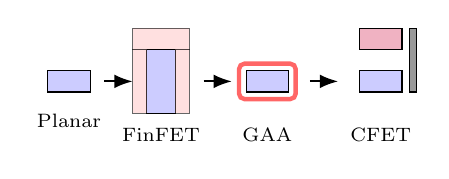
\begin{tikzpicture}[scale=0.9,>=Latex]
% simplified evolution schematic
\draw[fill=blue!20] (0,0) rectangle (0.6,0.3); % Planar
\node at (0.3,-0.4) {\scriptsize Planar};
\draw[->,thick] (0.8,0.15)--(1.2,0.15);

\draw[fill=blue!20] (1.4,-0.3) rectangle (1.8,0.6); % Fin
\draw[fill=red!20,opacity=0.6] (1.2,0.6) rectangle (2.0,0.9);
\draw[fill=red!20,opacity=0.6] (1.2,-0.3) rectangle (1.4,0.6);
\draw[fill=red!20,opacity=0.6] (1.8,-0.3) rectangle (2.0,0.6);
\node at (1.6,-0.6) {\scriptsize FinFET};
\draw[->,thick] (2.2,0.15)--(2.6,0.15);

\draw[fill=blue!20] (2.8,0.0) rectangle (3.4,0.3);
\draw[draw=red!60, ultra thick, rounded corners=2pt] (2.7,-0.1) rectangle (3.5,0.4);
\node at (3.1,-0.6) {\scriptsize GAA};
\draw[->,thick] (3.7,0.15)--(4.1,0.15);

\draw[fill=blue!20] (4.4,0.0) rectangle (5.0,0.3); % nFET
\draw[fill=blue!20!red!30] (4.4,0.6) rectangle (5.0,0.9); % pFET
\draw[fill=black!40] (5.1,0.0) rectangle (5.2,0.9); % via
\node at (4.7,-0.6) {\scriptsize CFET};
\end{tikzpicture}}
\caption{Device evolution schematic: Planar $\rightarrow$ FinFET (3-side) $\rightarrow$ GAA (4-side) $\rightarrow$ CFET (stacked n/p).}
\label{fig:evolution}
\end{figure}

% =========================
\begin{table}[t]
\centering
\caption{Technology Node Evolution: From GAA to CFET}
\label{tab:node_scaling}
\begin{tabular}{lcccc}
\hline
Node & Device & VDD & Density & Notes \\
\hline
7\,nm (2018)  & FinFET   & 0.70--0.80 & 90--100 & EUV, cell height limits \\
5\,nm (2020)  & FinFET$\to$pre-GAA & 0.65--0.75 & 130--170 & RC delay dominates \\
3\,nm (2023)  & GAA      & 0.60--0.70 & 200--250 & Four-sided control \\
2\,nm (2025e) & GAA prod.& 0.55--0.65 & 300--400 & Multi-sheet, DTCO \\
$<$2\,nm (27--) & CFET   & 0.50--0.60 & 500--700 & Cross-sectional inverter \\
1\,nm+ (2030+) & Seq./Forksheet & $<$0.50 & $>$800 & 3D stack, AI-assisted \\
\hline
\end{tabular}
\end{table}

% =========================
\section{CFET Structural Concepts}
Two integration styles are considered, reflecting a likely roadmap progression:
first the \emph{Sequential CFET} as the initial implementation candidate,
and then the \emph{Forksheet CFET} as a possible successor if inter-tier
interference proves problematic.

\paragraph*{(i) Sequential CFET}
The first integration style expected in practice is the Sequential CFET.
Here, the nFET tier is fabricated first, followed by the pFET tier stacked
above it under a constrained thermal budget.
Selective epitaxy/etch and dielectric isolation are crucial, as is vertical
contact to the inverter output.
Because n- and p-devices are stacked in close proximity, concerns arise
regarding electrostatic coupling, vertical via parasitics, and thermal interference.

\begin{figure}[t]
\centering
\fitfig{%
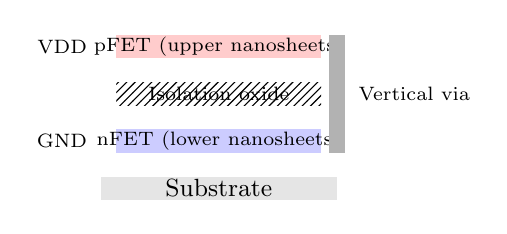
\begin{tikzpicture}[scale=1.0]
% Substrate
\fill[gray!20] (0,0) rectangle (3,0.3);
\node at (1.5,0.15) {\small Substrate};

% nFET
\fill[blue!20] (0.2,0.6) rectangle (2.8,0.9);
\node at (1.5,0.75) {\scriptsize nFET (lower nanosheets)};

% Isolation oxide
\fill[gray!40,pattern=north east lines] (0.2,1.2) rectangle (2.8,1.5);
\node at (1.5,1.35) {\scriptsize Isolation oxide};

% pFET
\fill[red!20] (0.2,1.8) rectangle (2.8,2.1);
\node at (1.5,1.95) {\scriptsize pFET (upper nanosheets)};

% Vertical via
\fill[black!30] (2.9,0.6) rectangle (3.1,2.1);
\node[anchor=west] at (3.15,1.35) {\scriptsize Vertical via};

% Supply labels
\node[anchor=east] at (-0.05,1.95) {\scriptsize VDD};
\node[anchor=east] at (-0.05,0.75) {\scriptsize GND};
\end{tikzpicture}}
\caption{Sequential CFET cross-section: stacked nFET/pFET with vertical output via.}
\label{fig:cfet_stack}
\end{figure}

\paragraph*{(ii) Forksheet CFET}
If interference in Sequential CFETs becomes too severe, a next-step option is the
Forksheet CFET.
In this style, n- and p-channels are placed orthogonally and separated by a dielectric
``fork'' spacer.
This geometry mitigates inter-tier parasitics, preserves electrostatic control,
and eases routing congestion.

\begin{figure}[t]
\centering
\fitfig{%
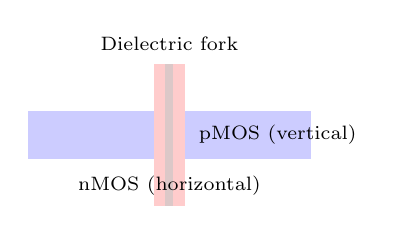
\begin{tikzpicture}[scale=1.0]
% nMOS horizontal
\fill[blue!20] (0.2,0.0) rectangle (3.8,0.6);
% pMOS vertical
\fill[red!20] (1.8,-0.6) rectangle (2.2,1.2);
% fork
\fill[gray!45,opacity=0.6] (1.95,-0.6) rectangle (2.05,1.2);

\node[anchor=south] at (2.00,1.25) {\scriptsize Dielectric fork};
\node[anchor=west]  at (2.25,0.30) {\scriptsize pMOS (vertical)};
\node[anchor=north] at (2.00,-0.10) {\scriptsize nMOS (horizontal)};
\end{tikzpicture}}
\caption{Forksheet CFET top view: orthogonal n/p nanosheets with dielectric fork.}
\label{fig:forksheet}
\end{figure}

% =========================
\section{Electrical and Layout Impacts}
CFET integration affects not only cell density but also delay,
variability, and power distribution in ways that extend beyond GAA devices.
Key educational points include:
\begin{itemize}
  \item \textbf{Area efficiency:} Vertical stacking nearly doubles inverter density.
  This extends to NAND/NOR cells by co-locating pull-up and pull-down networks in the same footprint.
  Implication: changes ripple into \emph{cell height} and \emph{routing pitch}.
  \item \textbf{Delay/energy:} Vertical n-to-p via shortens RC path vs.\ lateral wiring.
  Even with similar $I$–$V$ curves to GAA, FO1 delay and stage energy improve due to reduced interconnect length.
  \item \textbf{Electrostatics:} Each tier retains GAA-level control, but inter-tier dielectric coupling adds capacitance and via resistance.
  This highlights device–circuit parasitic interaction, a useful case for teaching multi-physics co-optimization.
  \item \textbf{Variability/noise:} Thermal coupling between tiers causes asymmetric heating.
  Partitioned VDD/GND networks generate uneven IR drop and noise susceptibility, driving new CAD and placement strategies.
\end{itemize}

% =========================
\section{Manufacturing Challenges}
Realizing CFETs requires overcoming unprecedented fabrication hurdles.
Independent n/p work-functions and junctions across stacked tiers demand selective epitaxy and etching, often under $<500^{\circ}$C budgets.
Vertical via alignment must achieve sub-5\,nm overlay, pushing EUV lithography beyond today’s standards.
Dielectric isolation must suppress dopant diffusion and preserve mechanical integrity.

IMEC demonstrations confirm Sequential CFET feasibility~\cite{imec_cfet_iedm2020}.
Yet industrial-scale yield, variability, and reliability remain unresolved.
Particularly, \emph{independent threshold-voltage tuning of nFET/pFET tiers} is essential for SRAM stability and logic integration.

% =========================
\section{Modeling and EDA Limitations}
Compact models such as BSIM-CMG capture GAA, but CFET extensions remain absent.
Key missing aspects include:
\begin{enumerate}
  \item Inter-tier electrostatics and capacitive coupling,
  \item Vertical thermal interactions between stacked devices,
  \item Parasitic RC from vertical vias and tier-to-tier contacts.
\end{enumerate}
Prototype Verilog-A models exist but lack calibration and reproducibility.
No open-source CFET-ready PDKs or libraries are available, preventing standardized flows.
This gap is echoed in IRDS~\cite{irds_2023}, making CFET a fertile topic for coursework and research.

% =========================
\section{Educational Value}
From a pedagogical view, CFET is more than a device—it is a framework linking physics, process, layout, and CAD.
Graduate courses may include:
\begin{itemize}
  \item Verilog-A CFET models as design projects,
  \item Sensitivity studies on inter-tier parasitics,
  \item Placement/routing co-optimization exercises,
  \item Roadmap-based DTCO (Design-Technology Co-Optimization) discussions.
\end{itemize}
Undergraduate courses can treat CFET as a case study in scaling limits, while advanced curricula can involve hands-on modeling and DTCO research.
This dual-level use illustrates how CFET bridges device-level abstraction and system-level design education.

% =========================
\section{Conclusion and Outlook}
CFET reframes CMOS as a stacked, cross-sectional inverter that simultaneously improves density and wiring delay.
Future research vectors include:
\begin{itemize}
  \item Forksheet layouts to mitigate inter-tier interference,
  \item 3D sequential stacks under constrained thermal budgets,
  \item Thermal-aware power partitioning across tiers,
  \item Co-optimized BEOL integration to cut parasitic loading,
  \item AI-driven exploration of DTCO design space.
\end{itemize}
Embedding CFET in curricula not only prepares engineers for the 2030s but cultivates critical thinking about unresolved scaling challenges.

% ========================
\section*{Acknowledgment}
The author thanks the Project Design Hub community for discussions.

% ========================
\bibliographystyle{IEEEtran}
\bibliography{refs}

% ========================
\section*{Author Biography}
\noindent\textbf{Shinichi Samizo}
received the M.S. degree in Electrical and Electronic Engineering from Shinshu University, Japan.
He worked at Seiko Epson Corporation on semiconductor memory and mixed-signal device development, and contributed to inkjet MEMS actuators and PrecisionCore printhead technology.
He is now an independent semiconductor researcher focusing on process/device education, memory architecture, and AI system integration.\\[2pt]
\textbf{Contact:} \href{mailto:shin3t72@gmail.com}{shin3t72@gmail.com}, \href{https://github.com/Samizo-AITL}{Samizo-AITL}

\end{document}
